\chapter{Introdução}

	
A Computação Ubíqua, \textit{ubicomp}, a tempos vem sendo tema de diversas
pesquisas ao redor do mundo. Mark Weiser diz que o computador do futuro deve ser
algo invisível, proporcionando ao usuário um melhor foco na tarefa. A Ubicomp
tenta atribuir tal invisibilidade aos computadores criando uma realidade na qual
o computador se integra a ambientes físicos constituindo os ambientes
inteligentes que interagem com seus usuários e possuem uma ampla e transparente
interação entre dispositivos e serviços disponíveis. A estes ambientes
inteligentes é dado o nome de \textit{smart space}, cujo objetivo é auxiliar o
usuário em suas tarefas utilizando os recursos
disponíveis~\cite{fabriciobuzzeto,alegomes,weiser1, weiser2}.
	
Um ambiente inteligente pode ser composto por uma grande variedade de
dispositivos, que fornecem ao ambiente recursos. Para que estes se agreguem as
tarefas do usuário, a inteligência presente deve coordená-los de acordo com as
informações sobre o ambiente e sobre o usuário~\cite{fabriciobuzzeto}. Portanto,
informações como posição do usuário e sua respectiva identidade são de grande
valia para tornar possível a interação entre o usuário e os recursos presentes.
Um ambiente ubíquo capaz de obter tais informações, pode prover uma
personalização automática de acordo com as preferências do usuário e até mesmo
prover um ambiente mais seguro com controle de acesso físico e prevenção de
fraudes \cite{saocarlos}.
	
Informações como estas são um desafio a \textit{ubicomp} devido a alta
dinamicidade do ambiente, no qual usuários entram e saem a todo momento e interagem entre si e
com diversos equipamentos. Com a utilização de sistemas baseados em sensores é
possível obter dados sobre os usuários no ambiente, que podem ser utilizados em
tarefas como rastreamento, localização e identificação. Estas tarefas, em
conjunto, podem fornecer informações de contexto contendo as posições e as
identidades de cada usuário no ambiente.
	
Neste trabalho é proposto um sistema de reconhecimento facial, rastreamento e
localização de usuários em um ambiente inteligente afim de prover informações de
contexto ao Middleware \textit{uOS}~\cite{fabriciobuzzeto}. Tal sistema é chamado de Sistema TRUE
(\textit{Tracking and Recognizing Users in the Environment}) que utiliza o
sensor \textit{Kinect} da marca Microsoft como dispositivo de entrada. Este, por
sua vez, fornece imagens de cor e de profundidade ao sistema. O middleware \textit{uOS} é voltado para a adaptabilidade de serviços em ambientes inteligentes. Conforme apresentado na Figura~\ref{fig:uos}, o uOS atua como uma camada entre as aplicações e os \textit{drivers}. Cada \textit{driver} representa um conjunto de serviços providos por um dispositivo.

\begin{figure}[htb]
		\begin{center}
			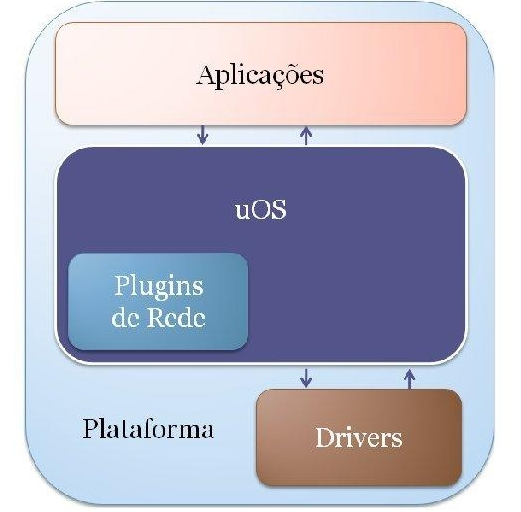
\includegraphics[scale=0.3]{figuras/1.Introducao/dsoa.jpg}
		\end{center}
		\caption{Middleware \textit{uOS}.}
		\label{fig:uos}
	\end{figure}

Este trabalho se encontra organizado da seguinte maneira. No
Capítulo~\ref{cap:fundamentacao} é apresentado conceitos e técnicas sobre
rastreamento de entidades, localização e identificação das mesmas em um ambiente
inteligente, além dos principais desafios da área. No
Capítulo~\ref{cap:trabalhos_correlatos} são analisados alguns projetos
relacionados ao rastreamento, a identificação e a localização de pessoas em um
ambiente inteligente. O trabalho desenvolvido é apresentado no
Capítulo~\ref{cap:true}, em que são descritos as diferentes etapas da
implementação do Sistema TRUE e as soluções utilizadas para realizar
rastreamento, localização e identificação de pessoas. Neste capítulo também é
descrita em detalhes como a integração do sistema com o Middleware \textit{uOS}
foi implementada. No Capítulo~\ref{cap:testes}, são apresentados os resultados
dos testes realizados para validar a implementação do Sistema TRUE. Por fim, no
Capítulo~\ref{cap:conclusao} são apresentados as considerações finais sobre este
trabalho bem como sugestões de trabalhos futuros.


